\documentclass[aspectratio=169]{beamer}

\mode<presentation>
{
  \usetheme{Singapore}
  \usecolortheme{default}
  \usefonttheme{default}
  \setbeamertemplate{navigation symbols}{}
  \setbeamertemplate{caption}[numbered]
  \setbeamertemplate{footline}[frame number]
}

\usepackage[french]{babel}
\usepackage{subcaption}
\usepackage[T1]{fontenc}
\usepackage[utf8]{inputenc}
\usepackage{tikz-qtree}
\usepackage[thinlines]{easytable}
\usepackage{siunitx}
\usepackage{calc}
\usepackage{multicol}
\usepackage{graphicx}
\usepackage{xcolor}
\usepackage{verbatim}
\usepackage{textcomp}
\usepackage{chngpage}
\usepackage{csquotes}
\usepackage{pgfplots}
\usepackage{pgf-umlsd}
\usepackage[backend=biber]{biblatex}
\usepackage{pgfplots}
\usepackage{pgf-umlsd}
\addbibresource{synthese.bib}
\usetikzlibrary{arrows}

\title{Développement d'une solution cryptographique permettant de vérifier la présence ou l'absence à un événement}
\subtitle{Soutenance de fin de projet}
\author[me]{Thibault de Boutray, Louis Vignier\\[2mm]Encadrant : Christophe Bidan}
\institute{CentraleSupélec}
\date{26 mars 2020}

\AtBeginSubsection[]
{
  \begin{frame}
  \frametitle{Sommaire}
  \tableofcontents[currentsubsection]
  \end{frame}
}

\AtBeginSubsection[]
{
  \begin{frame}
  \frametitle{Sommaire}
  \tableofcontents[currentsubsection]
  \end{frame}
}

\begin{document}

\begin{frame}
  \titlepage
\end{frame}

\begin{frame}{Plan}
  \tableofcontents
\end{frame}

\section{Introduction}

\subsection{Présentation du sujet}

\begin{frame}{Problématique}
	Comment vérifier la présence effective d'un utilisateur à un événement, et dans la durée ?
	
	\bigskip
	
	\begin{itemize}
        \item Présence en réunion, en cours, à une conférence
        \item Vérification effectuée par le Maître de Conférence (MDC)
	\end{itemize}

\end{frame}

\begin{frame}{Cahier des Charges}
  \begin{itemize}
    \item Assurer la présence d’un utilisateur à un événement	
    \begin{itemize}
      \item Vérification ponctuelle ou sur la durée complète de l'événement\pause
    \end{itemize}
    \item Propriétés d'utilisation
    \begin{itemize}
      \item Simple d’utilisation pour les maîtres de conférence
      \item Supporte $\sim$~150 participants et portée jusqu'à \SI{150}{\meter}
      \item Peu d’actions de la part des participants
      \item Doit pouvoir fonctionner sur une journée entière
      \item Assure la présence effective et unique de l’utilisateur\pause
    \end{itemize}
    \item Propriétés de privacy
    \begin{itemize}
      \item Eviter le "flicage" (par ex. suivi non sollicité en arrière-plan)
      \item Respecter la réglementation en vigueur (RGPD)
      \item Avoir un mode "anonyme" avec un simple compte des participants pour réaliser des statistiques (choisi par le MDC)
    \end{itemize}
  \end{itemize}
\end{frame}

\begin{frame}{Les attaques}
    \centering
\begin{tikzpicture}
    % Amphi
    \draw [black, thick, dotted] (0,0) circle [radius=3];
    \node [above] at (0,3) {Amphi};

    % Prof
    \draw [fill] (0,-0.2) circle [radius=0.05];
    \node [above] at (0,-0.2) {Prof};

    \pause

    % Eleve seul
    \draw [fill, gray] (4,0) circle [radius=0.05];
    \node [right, gray] at (4,0) {E};
    \draw [->, thick, line width=1.2, gray] (3.75,0) -- (0.5,0);
    \node [right, gray] at (6, 2) {Attaque au lit};

    \pause

    % Complicité interne
    \draw [fill, cyan] (1.3, -1.3) circle [radius=0.05];
    \node [above right, cyan] at (1.3, -1.3) {BP};
    \draw [fill, cyan] (3,-3) circle [radius=0.05];
    \node [right, cyan] at (3,-3) {E};
    \draw [->, thick, dashed, line width=1.2, cyan] (2.85,-2.85) -- (1.45,-1.45);
    \draw [->, thick, line width=1.2, cyan] (1.15,-1.15) -- (0.35,-0.35);
    \node [right, cyan] at (6, 1) {Attaque relai (complice)};

    \pause

    % Sans complicité
    \draw [fill, orange] (1.3, 1.3) circle [radius=0.05];
    \node [below right, orange] at (1.3, 1.3) {A};
    \draw [fill, orange] (3,3) circle [radius=0.05];
    \node [right, orange] at (3,3) {E};
    \draw [->, thick, dashed, line width=1.2, orange] (2.85,2.85) -- (1.45,1.45);
    \draw [->, thick, line width=1.2, orange] (1.15,1.15) -- (0.35,0.35);
    \node [right, orange] at (6, 0) {Attaque relai (tiers abusé)};

    \pause

    % Pokemon
    \draw [red, thick] (-1.3,-1.3) circle [radius=0.5];
    \node [right, red] at (-0.8, -1.3) {BP};
    \draw [fill, red] (-1.1,-1.3) circle [radius=0.05];
    \draw [fill, red] (-1.3,-1.3) circle [radius=0.05];
    \draw [fill, red] (-1.5,-1.3) circle [radius=0.05];
    \draw [fill, red] (-1.3,-1.5) circle [radius=0.05];
    \draw [fill, red] (-1.3,-1.1) circle [radius=0.05];
    \draw [->, thick, line width=1.2, red] (-0.94,-0.94) -- (-0.35,-0.35);
    \node [right, red] at (6, -1) {Attaque Pokemon\texttrademark};

    \pause

    % sybil
    \draw [fill, olive] (-1.3,1.3) circle [radius=0.05];
    \node [above left, olive] at (-1.3, 1.3) {BP};
    \draw [->, thick, line width=1.2, olive] (-1.15,1.35) to [out=15,in=105] (-0.15,0.45);
    \draw [->, thick, line width=1.2, olive] (-1.35,1.15) to [out=255,in=165] (-0.45,0.15);
    \node [right, olive] at (6, -2) {Attaque Sybil};
\onslide<1->
\end{tikzpicture}

\end{frame}

\subsection{Choix technologiques}

\begin{frame}{Résumé des études préliminaires}

\begin{table}[]
\begin{tabular}{|l|l|l|}
\hline
\textbf{Technologie} & \textbf{Avantages}                                                                              & \textbf{Inconvénients}                                                                            \\ \hline
RFID                 & \begin{tabular}[c]{@{}l@{}}Portée qui peut être adaptée \\ en fonction du protocole\end{tabular} & Pas présent dans tous les device                                                                  \\ \hline
NFC                  & \begin{tabular}[c]{@{}l@{}}Très simple à implémenter\\ Sécurité physique\end{tabular}           & Portée très courte                                                                                \\ \hline
Bluetooth            & Portée Idéale                                                                                   & \begin{tabular}[c]{@{}l@{}}Pas du tout adapté pour  \\ plusieurs devices\end{tabular}          \\ \hline
Wi-Fi                & \begin{tabular}[c]{@{}l@{}}Portée Idéale\\ Ok pour plusieurs device\end{tabular}                & \begin{tabular}[c]{@{}l@{}}Collisions\\ Traverse les murs\\ À délimiter avec des PDD\end{tabular} \\ \hline
\end{tabular}
\end{table}

\end{frame}

\begin{frame}{Choix Technologiques Globaux}

  Solution hybride à base de Wi-Fi, de son et de NFC :
  \begin{itemize}
      \item NFC pour vérifier l'entrée et la sortie des élèves dans la salle
      \item Wi-Fi et son pour vérifier la présence effective pendant le cours (PDD)
      \item Modularité pour le MDC : permettrait de choisir la vérification permanente ou juste à l'entrée et la sortie
  \end{itemize}
  
\end{frame}
  
\begin{frame}{Mesure de distance équivalente}
          
      Programme en C++ permettant de tester avec un ping :
      \begin{itemize}
          \item Localhost
          \begin{itemize}
              \item Min : \SI{3}{\kilo\meter} 
              \item Moyenne : \SI{10}{\kilo\meter} 
          \end{itemize}
          \item Routeur d'une résidence étudiante
          \begin{itemize}
              \item Min : \SI{100}{\kilo\meter} 
              \item Moyenne : \SI{140}{\kilo\meter} 
          \end{itemize}
      \end{itemize}

      \bigskip

      Implémentation du Swiss-Knife en localhost :
      \begin{itemize}
          \item Min : \SI{24}{\kilo\meter} 
          \item Moyenne : \SI{39}{\kilo\meter} 
      \end{itemize}
  
\end{frame}

\begin{frame}{Architecture du système}
  \centering
  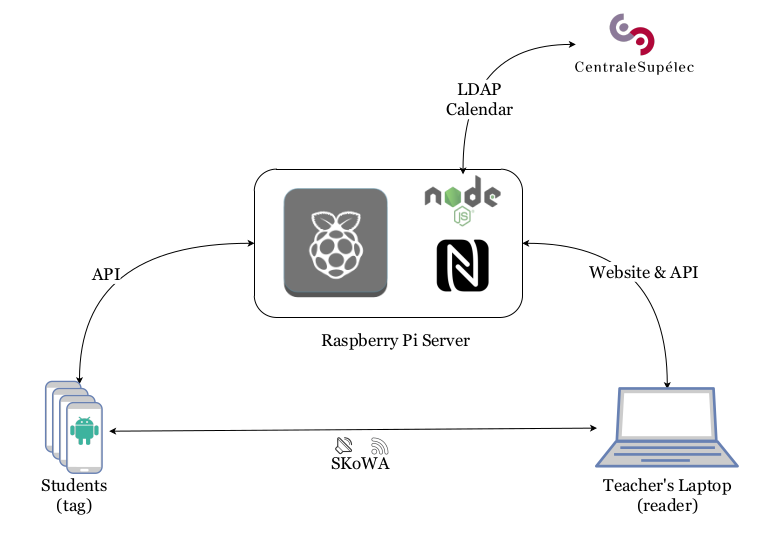
\includegraphics[height=0.8\textheight]{../assets/architecture.png}
\end{frame}


\section{Raspberry Pi}

\begin{frame}{Présentation}
  Le raspberry Pi a plusieurs utilités dans notre projet, et sert de serveur pour certains composants.
  \begin{itemize}
    \item Lecteur NFC géré par une librairie python (NxpPy)
    \item Backend de l'application web (node JS)
    \item Base de donnée (SQLite3 pour le développement)
    \item Parsing du LDAP de CentraleSupélec puis écriture dans la DB
  \end{itemize}

  \begin{figure}
    \begin{subfigure}{.2\textwidth}
      \centering
      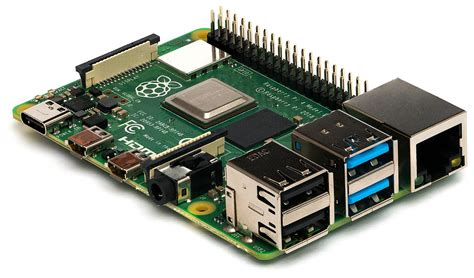
\includegraphics[width=.8\linewidth]{../assets/raspi.jpeg}
    \end{subfigure}
    \begin{subfigure}{.2\textwidth}
      \centering
      
\includegraphics[width=.8\linewidth]{../assets/nfc.png}
    \end{subfigure}
    \begin{subfigure}{.2\textwidth}
      \centering
      
\includegraphics[width=.8\linewidth]{../assets/nodejs.png}
    \end{subfigure}
  \end{figure}
\end{frame}

\subsection{NFC}

\begin{frame}{Présentation NFC}
  Nous avons utilisé le module \textit{explore-nfc} de la société NXP qui se branche sur les GPIO du raspberry PI
  \begin{figure}. 
      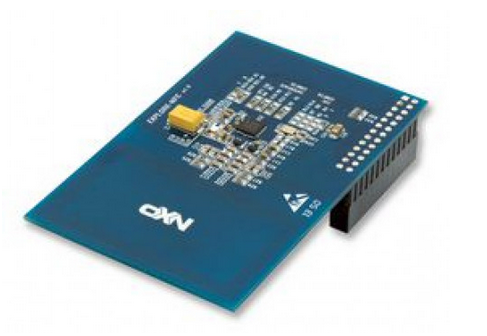
\includegraphics[width=.5\textwidth]{../assets/explorenfc.png}
  \end{figure}  
\end{frame} 

\begin{frame}{Fonctionnement du NFC}
  2 Scripts Python3 :
  \begin{itemize}
    \item Un script de polling qui interface avec le module NFC grâce à la librairie \textbf{NxpPY}, et qui communique avec le frontweb grâce à des websockets
    \item Un script \textit{Database Utils} qui interface avec la base de donnée \textbf{Sqlite3}
  \end{itemize}
  \begin{figure}
    \centering
    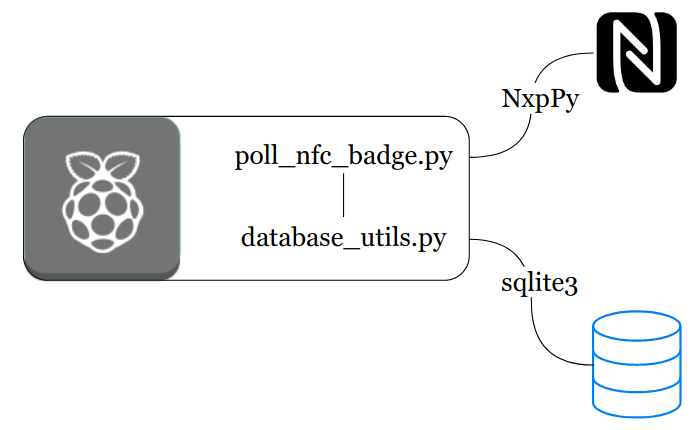
\includegraphics[width=.5\textwidth]{../assets/nfcarchitecture.png}
  \end{figure}
\end{frame}

\begin{frame}{poll\_nfc\_badge.py}
  Ce script utilise la librairie \textit{websockets} de Python3, qui est elle même basée sur \textit{asyncio} qui permet de faire de la programmation asynchrone
  C'est le front end qui envoie au serveur ce dont il a besoin :
  \begin{itemize}
    \item Type = 0 $\rightarrow$ Check Once (à l'ajout d'un utilisateur, permet de scanner le badge une fois)
    \item Type = 1 $\rightarrow$ Vérification à l'entrée dans l'amphi
    \item Type = 2 $\rightarrow$ Vérification à la sortie de l'amphi
  \end{itemize}

\end{frame}

\begin{frame}{Type 0 (Check Once)}
  \begin{figure}[]
    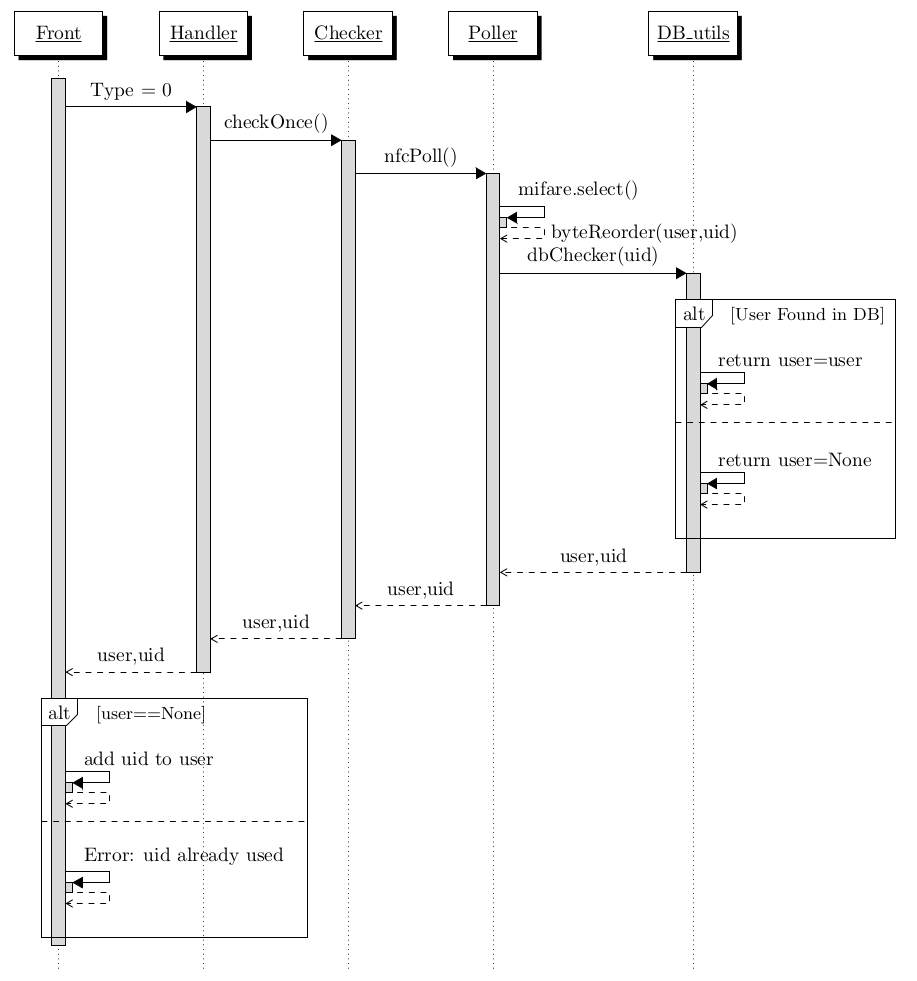
\includegraphics[height=\textheight]{../assets/nfcSeqOnce.png}
  \end{figure}

\end{frame}

\begin{frame}{Type 1 (Verification à l'entrée)}
  \begin{figure}[]
    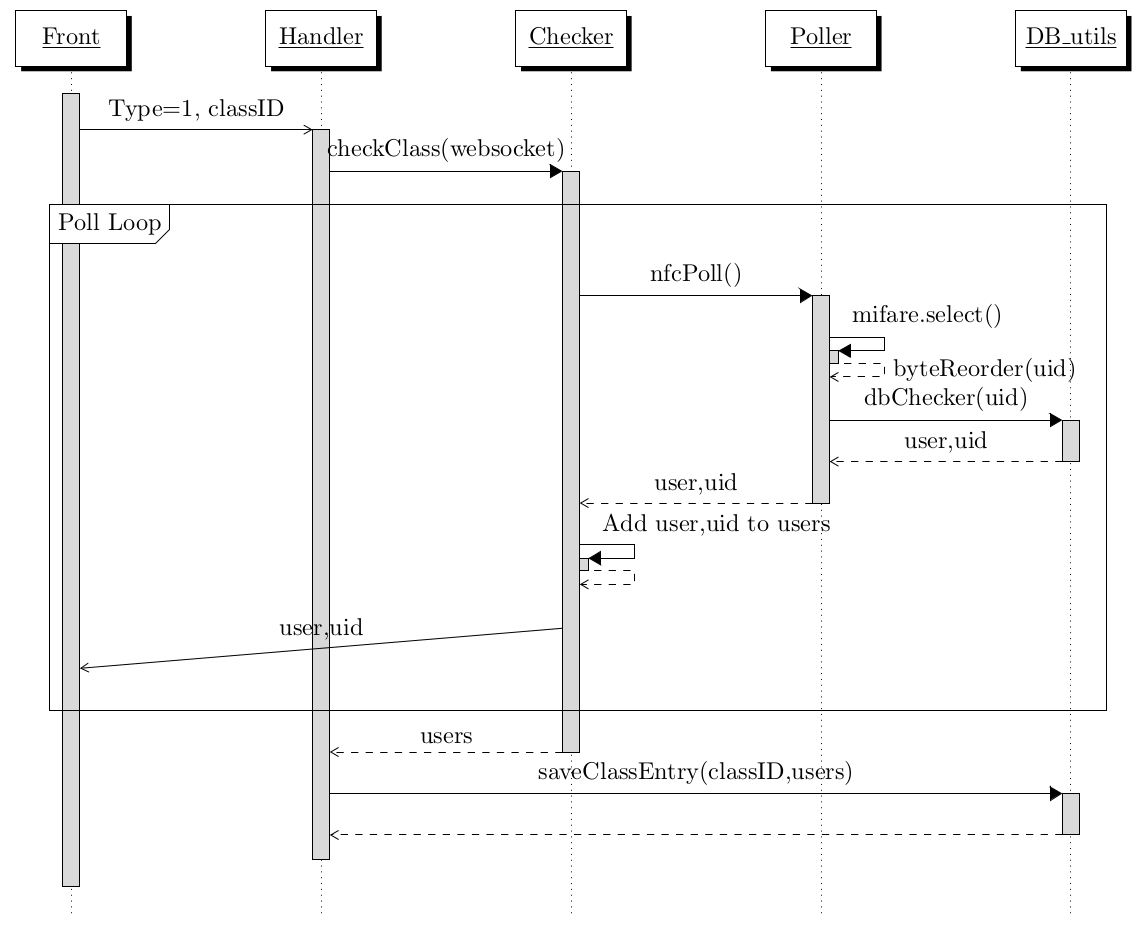
\includegraphics[height=\textheight]{../assets/nfcSeqEntry.png}
  \end{figure}

\end{frame}

\begin{frame}{Type 2 (Vérification à la sortie)}
  \begin{figure}[]
    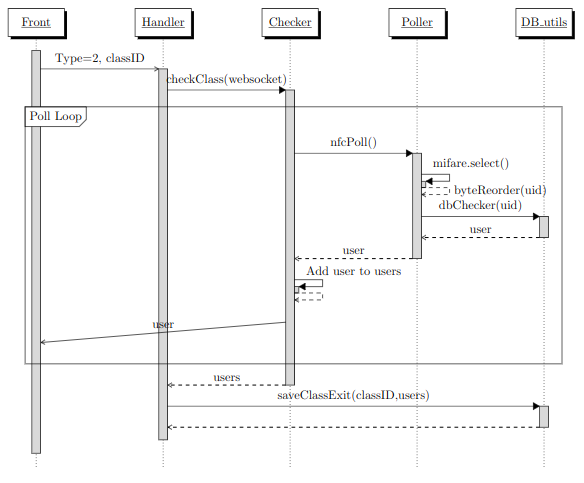
\includegraphics[height=\textheight]{../assets/nfcSeqExit.png}
  \end{figure}

\end{frame}

\subsection{Application Web}

\begin{frame}{Présentation de l'appli Web}  

\end{frame}

\begin{frame}{Architecture de l'appli Web}  

\end{frame}



\subsection{LDAP Parser}

\begin{frame}{Présentation}  

\end{frame}

\begin{frame}{Champs récupérés}  

\end{frame}

\section{SKoWA}

\subsection{Swiss-Knife}

\begin{frame}{Le protocole Swiss-Knife}
  Protocole délimiteur de distance proposé en 2008. \cite{SwissKnife}

  \bigskip

  \begin{itemize}
    \item Authentification
    \item Résistance aux mafia fraud et terrorist fraud
    \item Faible complexité algorithmique
    \item Faible taux de faux positifs
    \item Confidentialité
    \item Résistance aux erreurs
  \end{itemize}
\end{frame}

\begin{frame}{Le protocole Swiss-Knife}
  
  \centering
  \begin{tikzpicture}

      % Partie 1
      \draw (-3, 2) rectangle (3, 0.5);
      \node [above, blue] at (0, 1.25) {Phase de préparation};
      \node at (0, 1) {Initialisation, réponses};


      \draw (-3, 0) rectangle (3, -1.5);
      \node [above, blue] at (0, -0.75) {Phase rapide};
      \node at (0, -1) {$m$ questions / réponses};

      \draw (-3, -2) rectangle (3, -3.5);
      \node [above, blue] at (0, -2.75) {Phase de vérification};
      \node at (0, -3) {Vérification};

  \onslide<1->
  \end{tikzpicture}

\end{frame}

\begin{frame}{Librairie .jar : Structure}
  Structure de la librairie
\end{frame}

\begin{frame}{Phase de préparation}
  \begin{multicols}{2}
    \begin{minipage}[c]{\linewidth}
      \centering
      \bigskip
      \medskip
      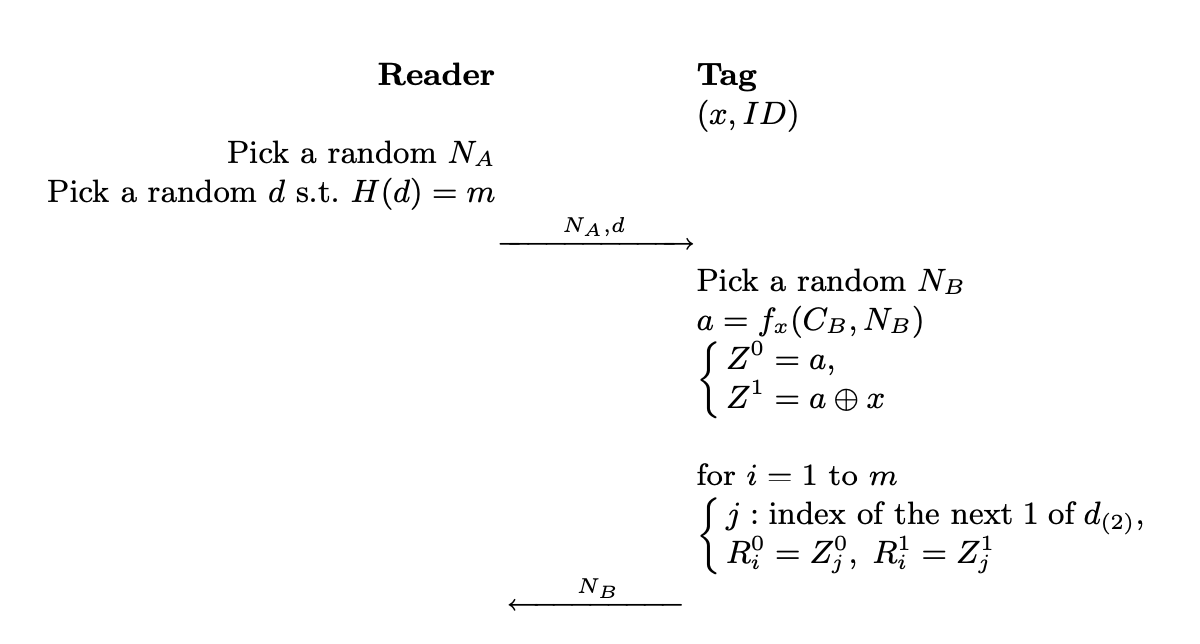
\includegraphics[width=\linewidth]{../assets/sk-phase1.png}
    \end{minipage}

    \begin{minipage}[t]{\linewidth}
      \begin{enumerate}
        \item Le lecteur choisit un nonce $N_A$, et $d$ un nombre avec $m$ bits 1.
        \item Le tag choisit un nonce $N_B$, et calcule $a = f_x(C_B, N_B)$ avec sa clé secrète $x$ et $N_B$. ($C_B$ est une constante)
        \item Le tag calcule $Z_0 = a$, $Z_1 = a \oplus x$. Il prépare ensuite les réponses possibles $R_0$ et $R_1$ selon le masque $d$.
        \item Le tag envoie $N_B$ au lecteur.
      \end{enumerate}
    \end{minipage}
  \end{multicols}
\end{frame}

\begin{frame}{Phase rapide}
  \begin{figure}[!htb]
    \centering

    \begin{minipage}{.45\textwidth}
        \centering
        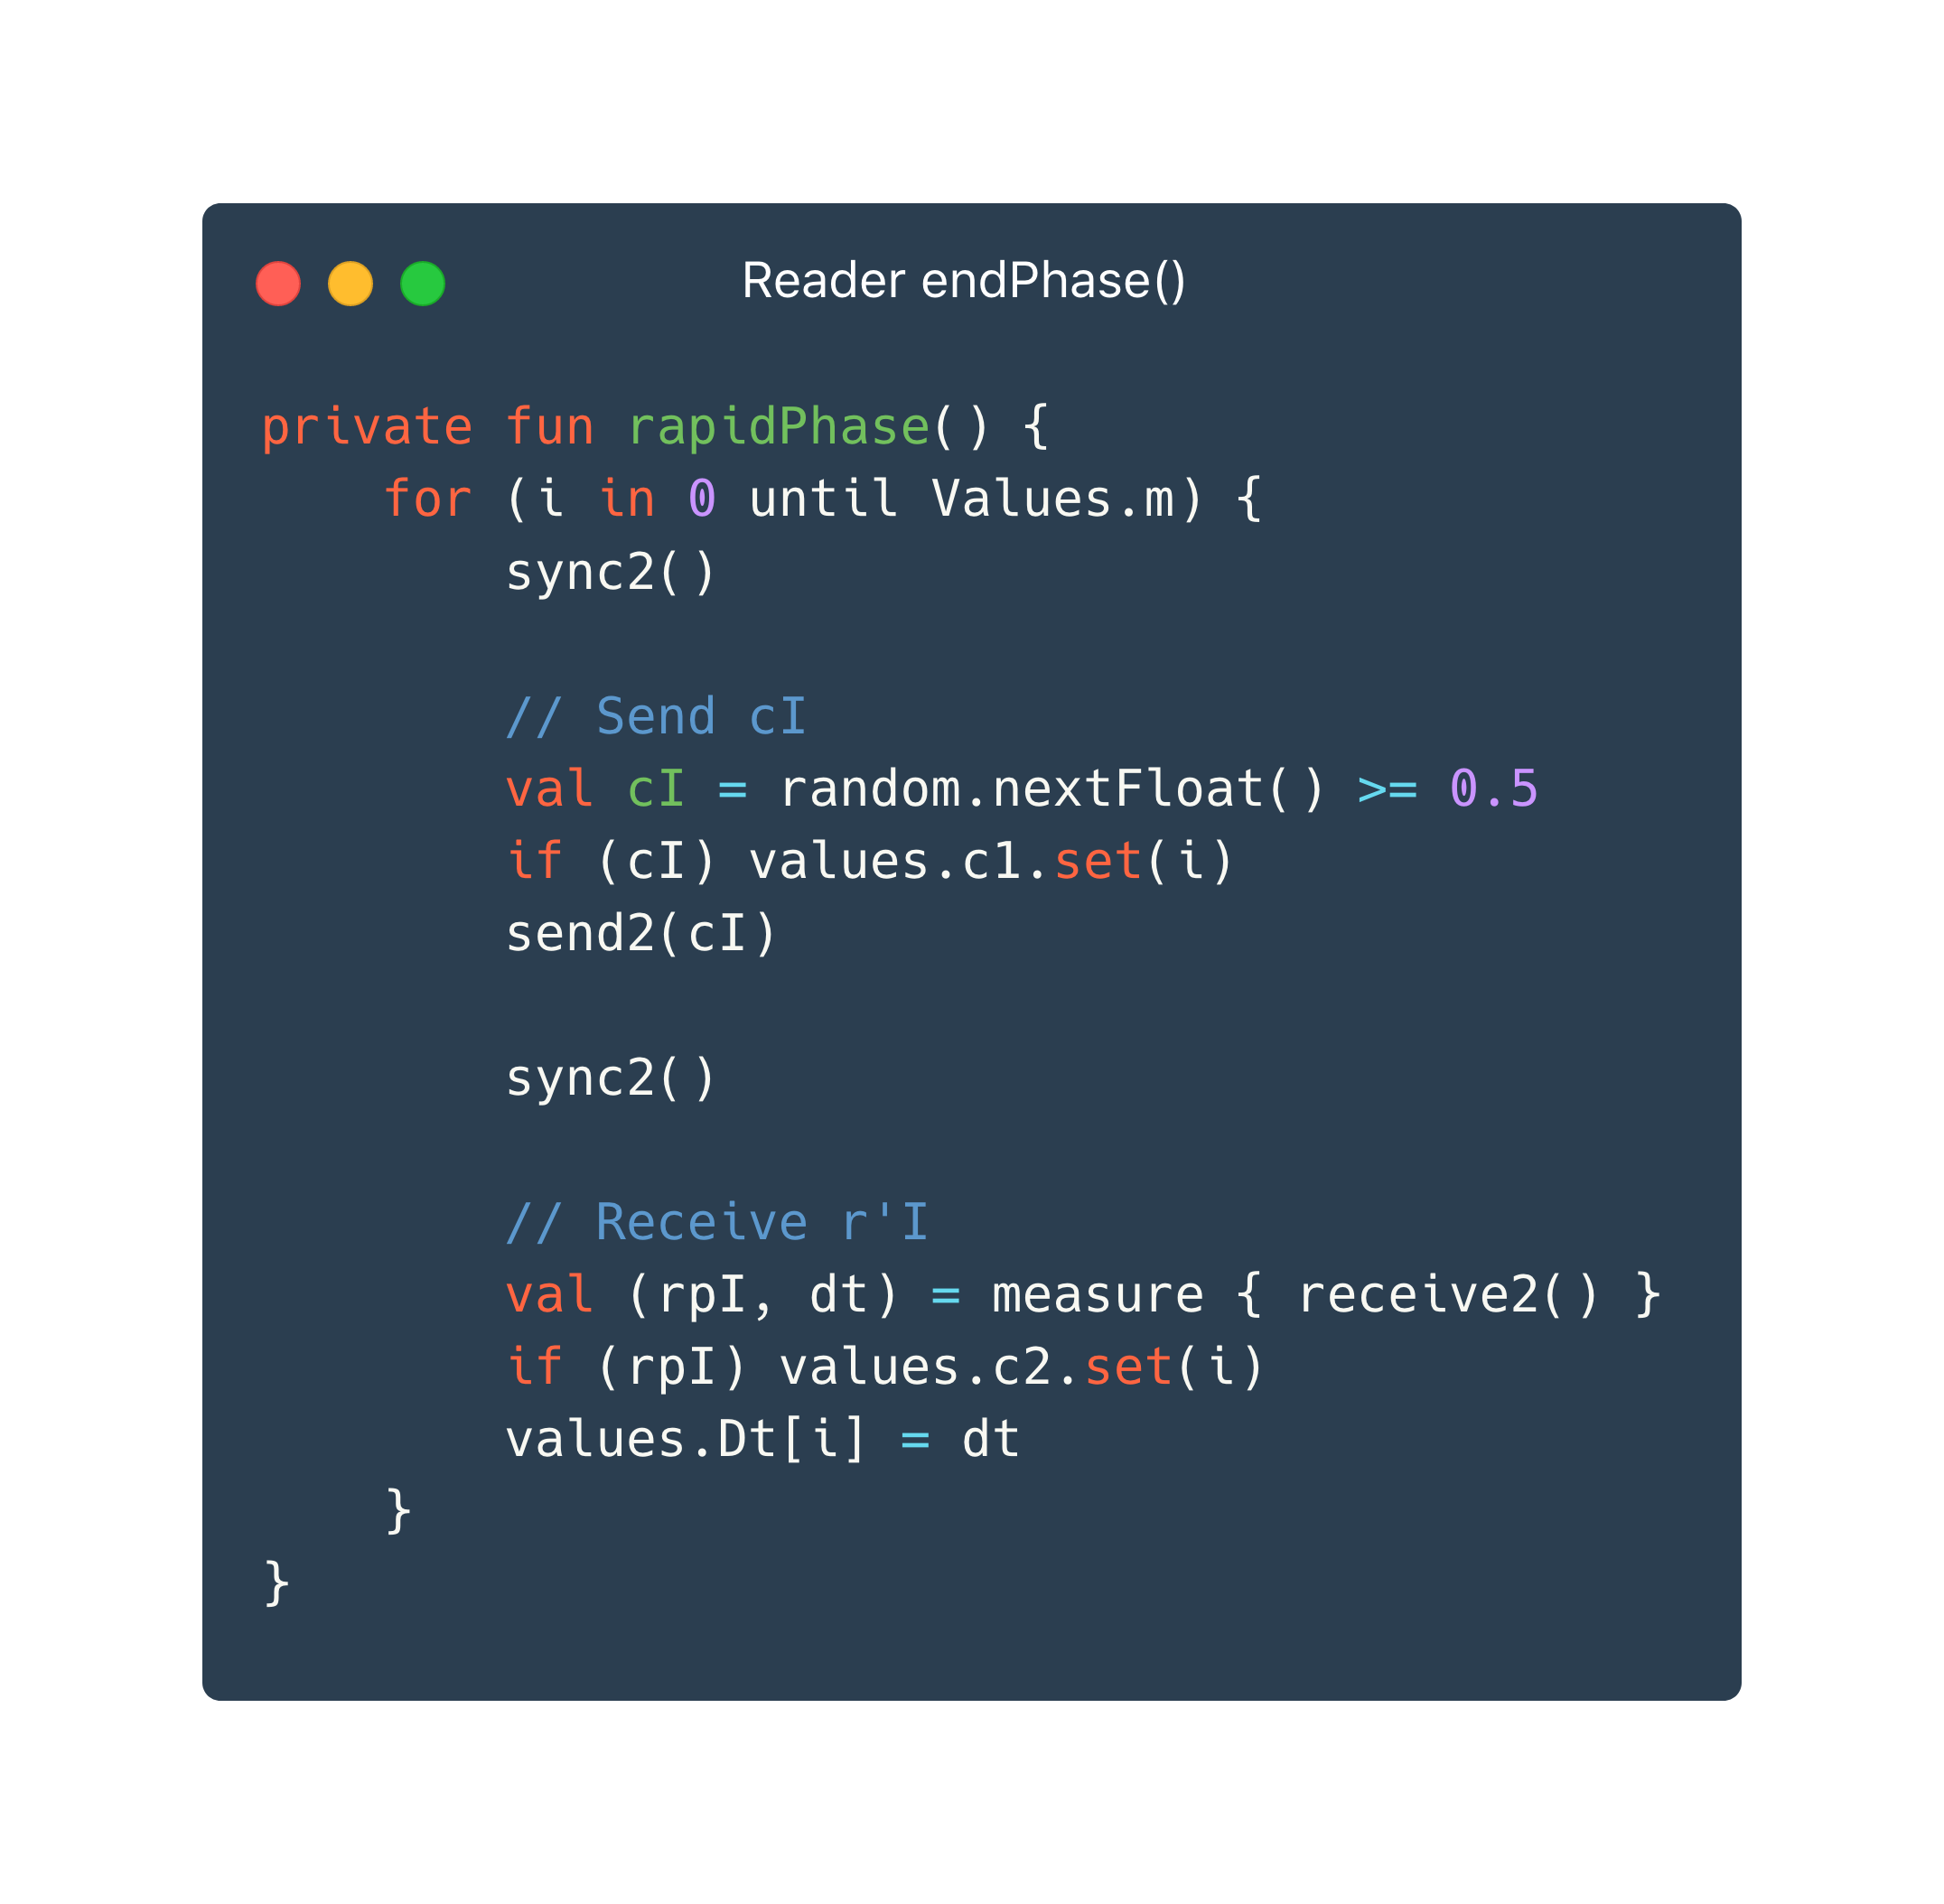
\includegraphics[width=\linewidth]{../assets/reader2}
    \end{minipage}%
    \begin{minipage}{.55\textwidth}
        \centering
        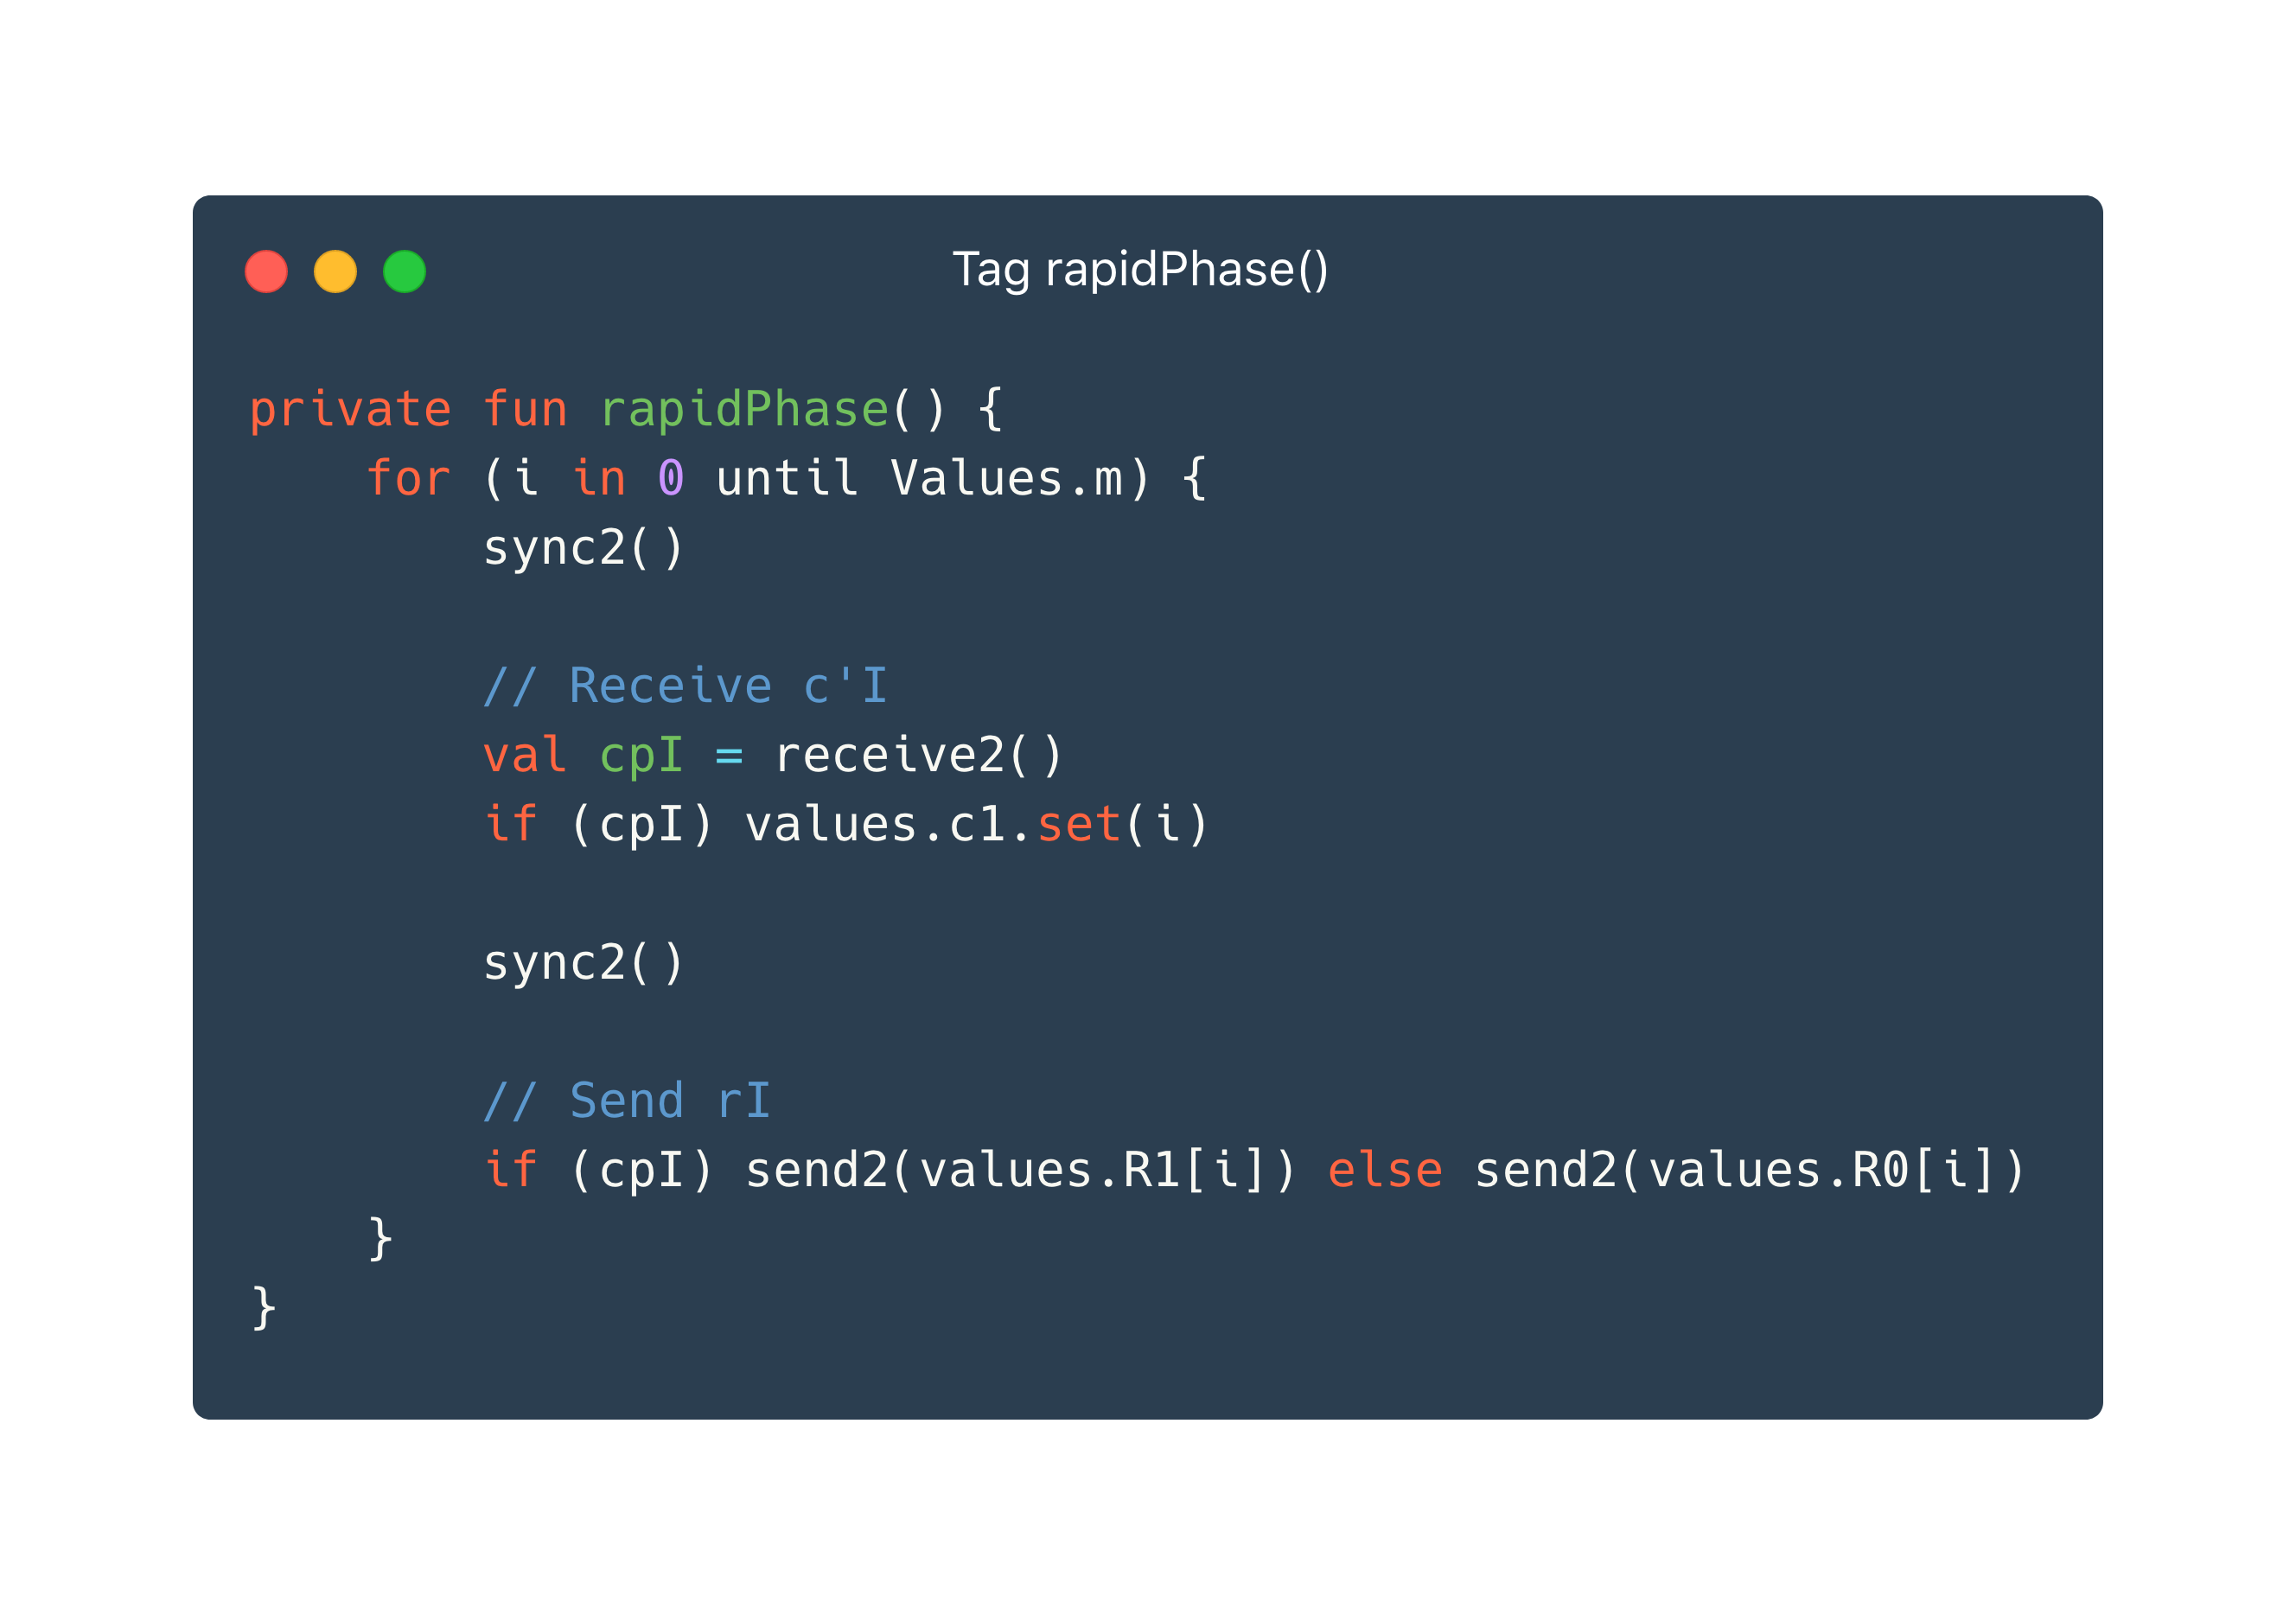
\includegraphics[width=\linewidth]{../assets/tag2}
    \end{minipage}

  \end{figure}
\end{frame}

\begin{frame}{Phase de vérification}
  \begin{multicols}{2}
    \begin{minipage}[c]{\linewidth}
      \centering
      \bigskip
      \bigskip
      \bigskip
      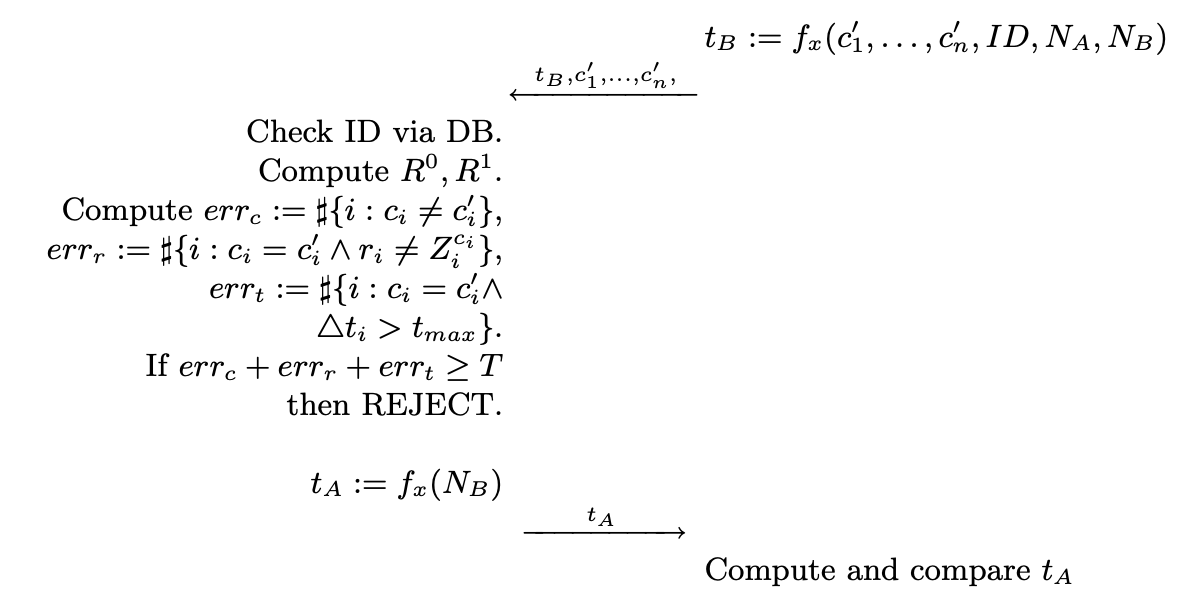
\includegraphics[width=\linewidth]{../assets/sk-phase3}
    \end{minipage}

    \begin{minipage}[t]{\linewidth}
      \begin{enumerate}
        \item Le tag envoie $t_B = f_x(c'_1, \hdots, c'_n, ID, N_A, N_B)$, et les $c'_i$.
        \item Le lecteur cherche dans sa base de tags jusqu'à trouver $(ID, x)$ générant $t_B$.
        \item Le lecteur calcule $R^0$ et $R^1$.
        \item Le lecteur compte les erreurs, si il y en a plus de $T$, échec.
        \item (optionnel) Le lecteur envoie $t_A := f_x(N_B)$ puis le tag le vérifie.
      \end{enumerate}
    \end{minipage}
  \end{multicols}
\end{frame}

\begin{frame}{Fonctions abstraites du Tag}
  \centering
  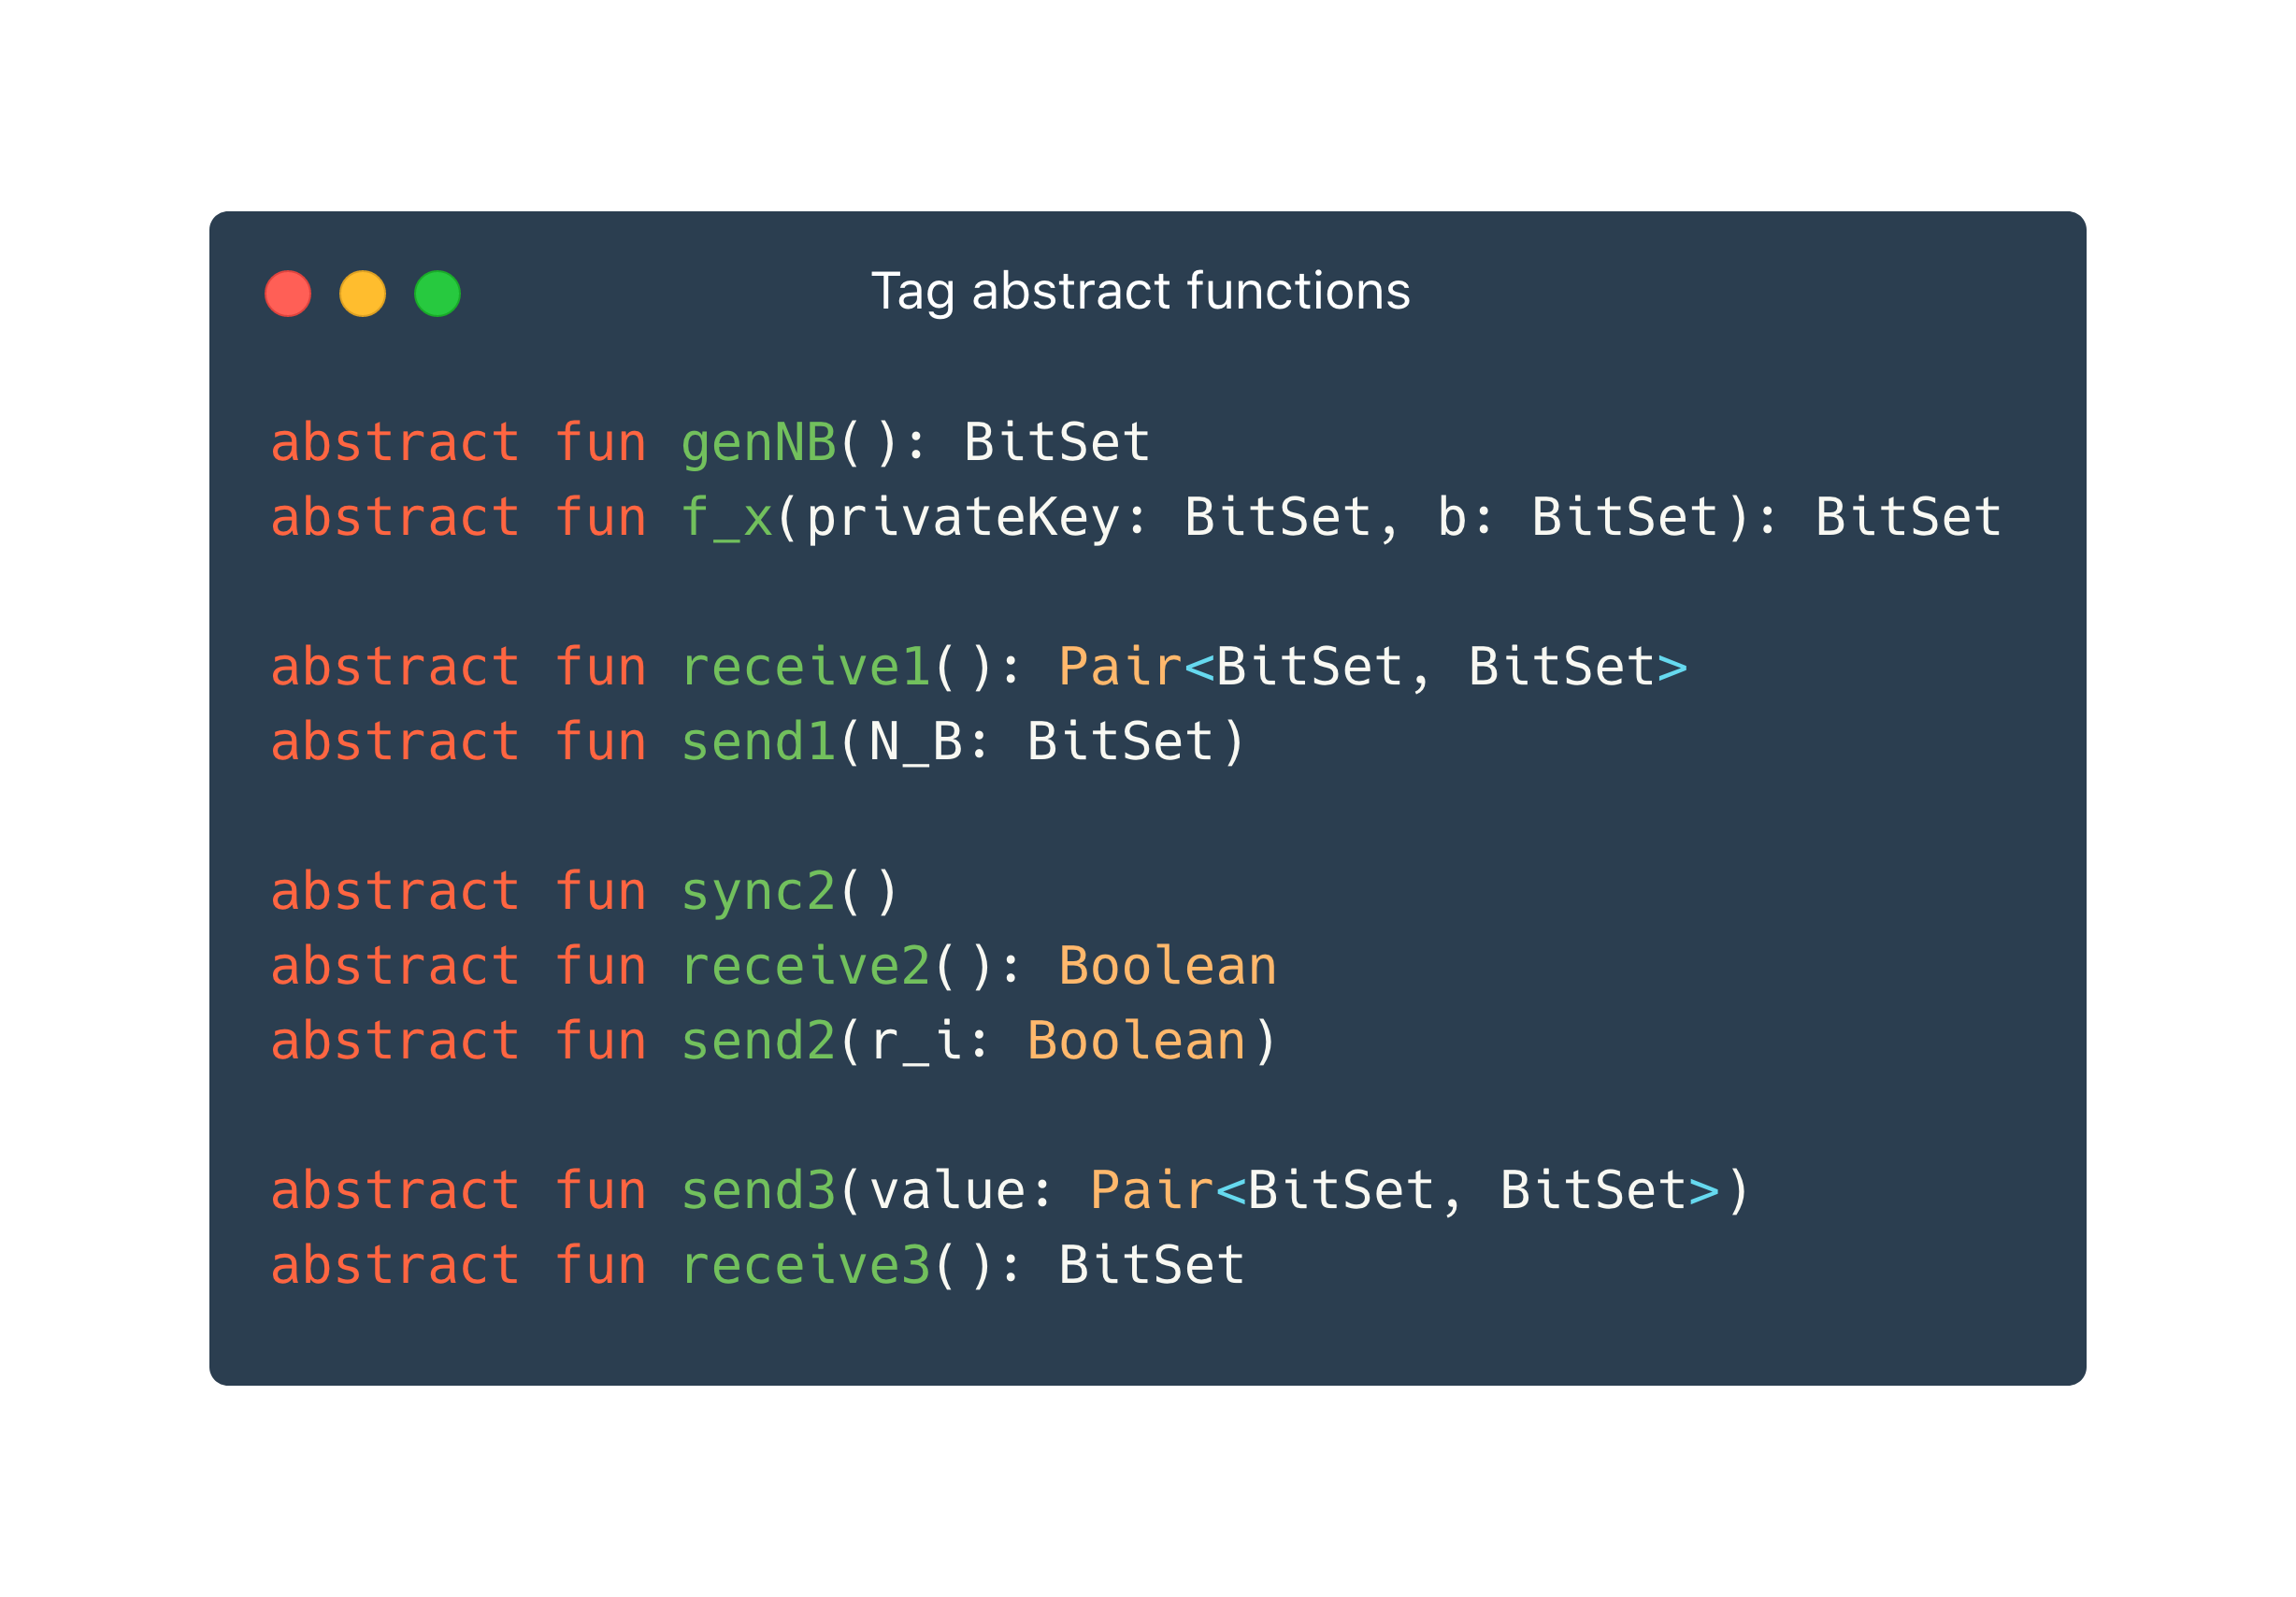
\includegraphics[width=.75\linewidth]{../assets/tagAbs}
\end{frame}

\begin{frame}{Fonctions abstraites du Reader}
  \centering
  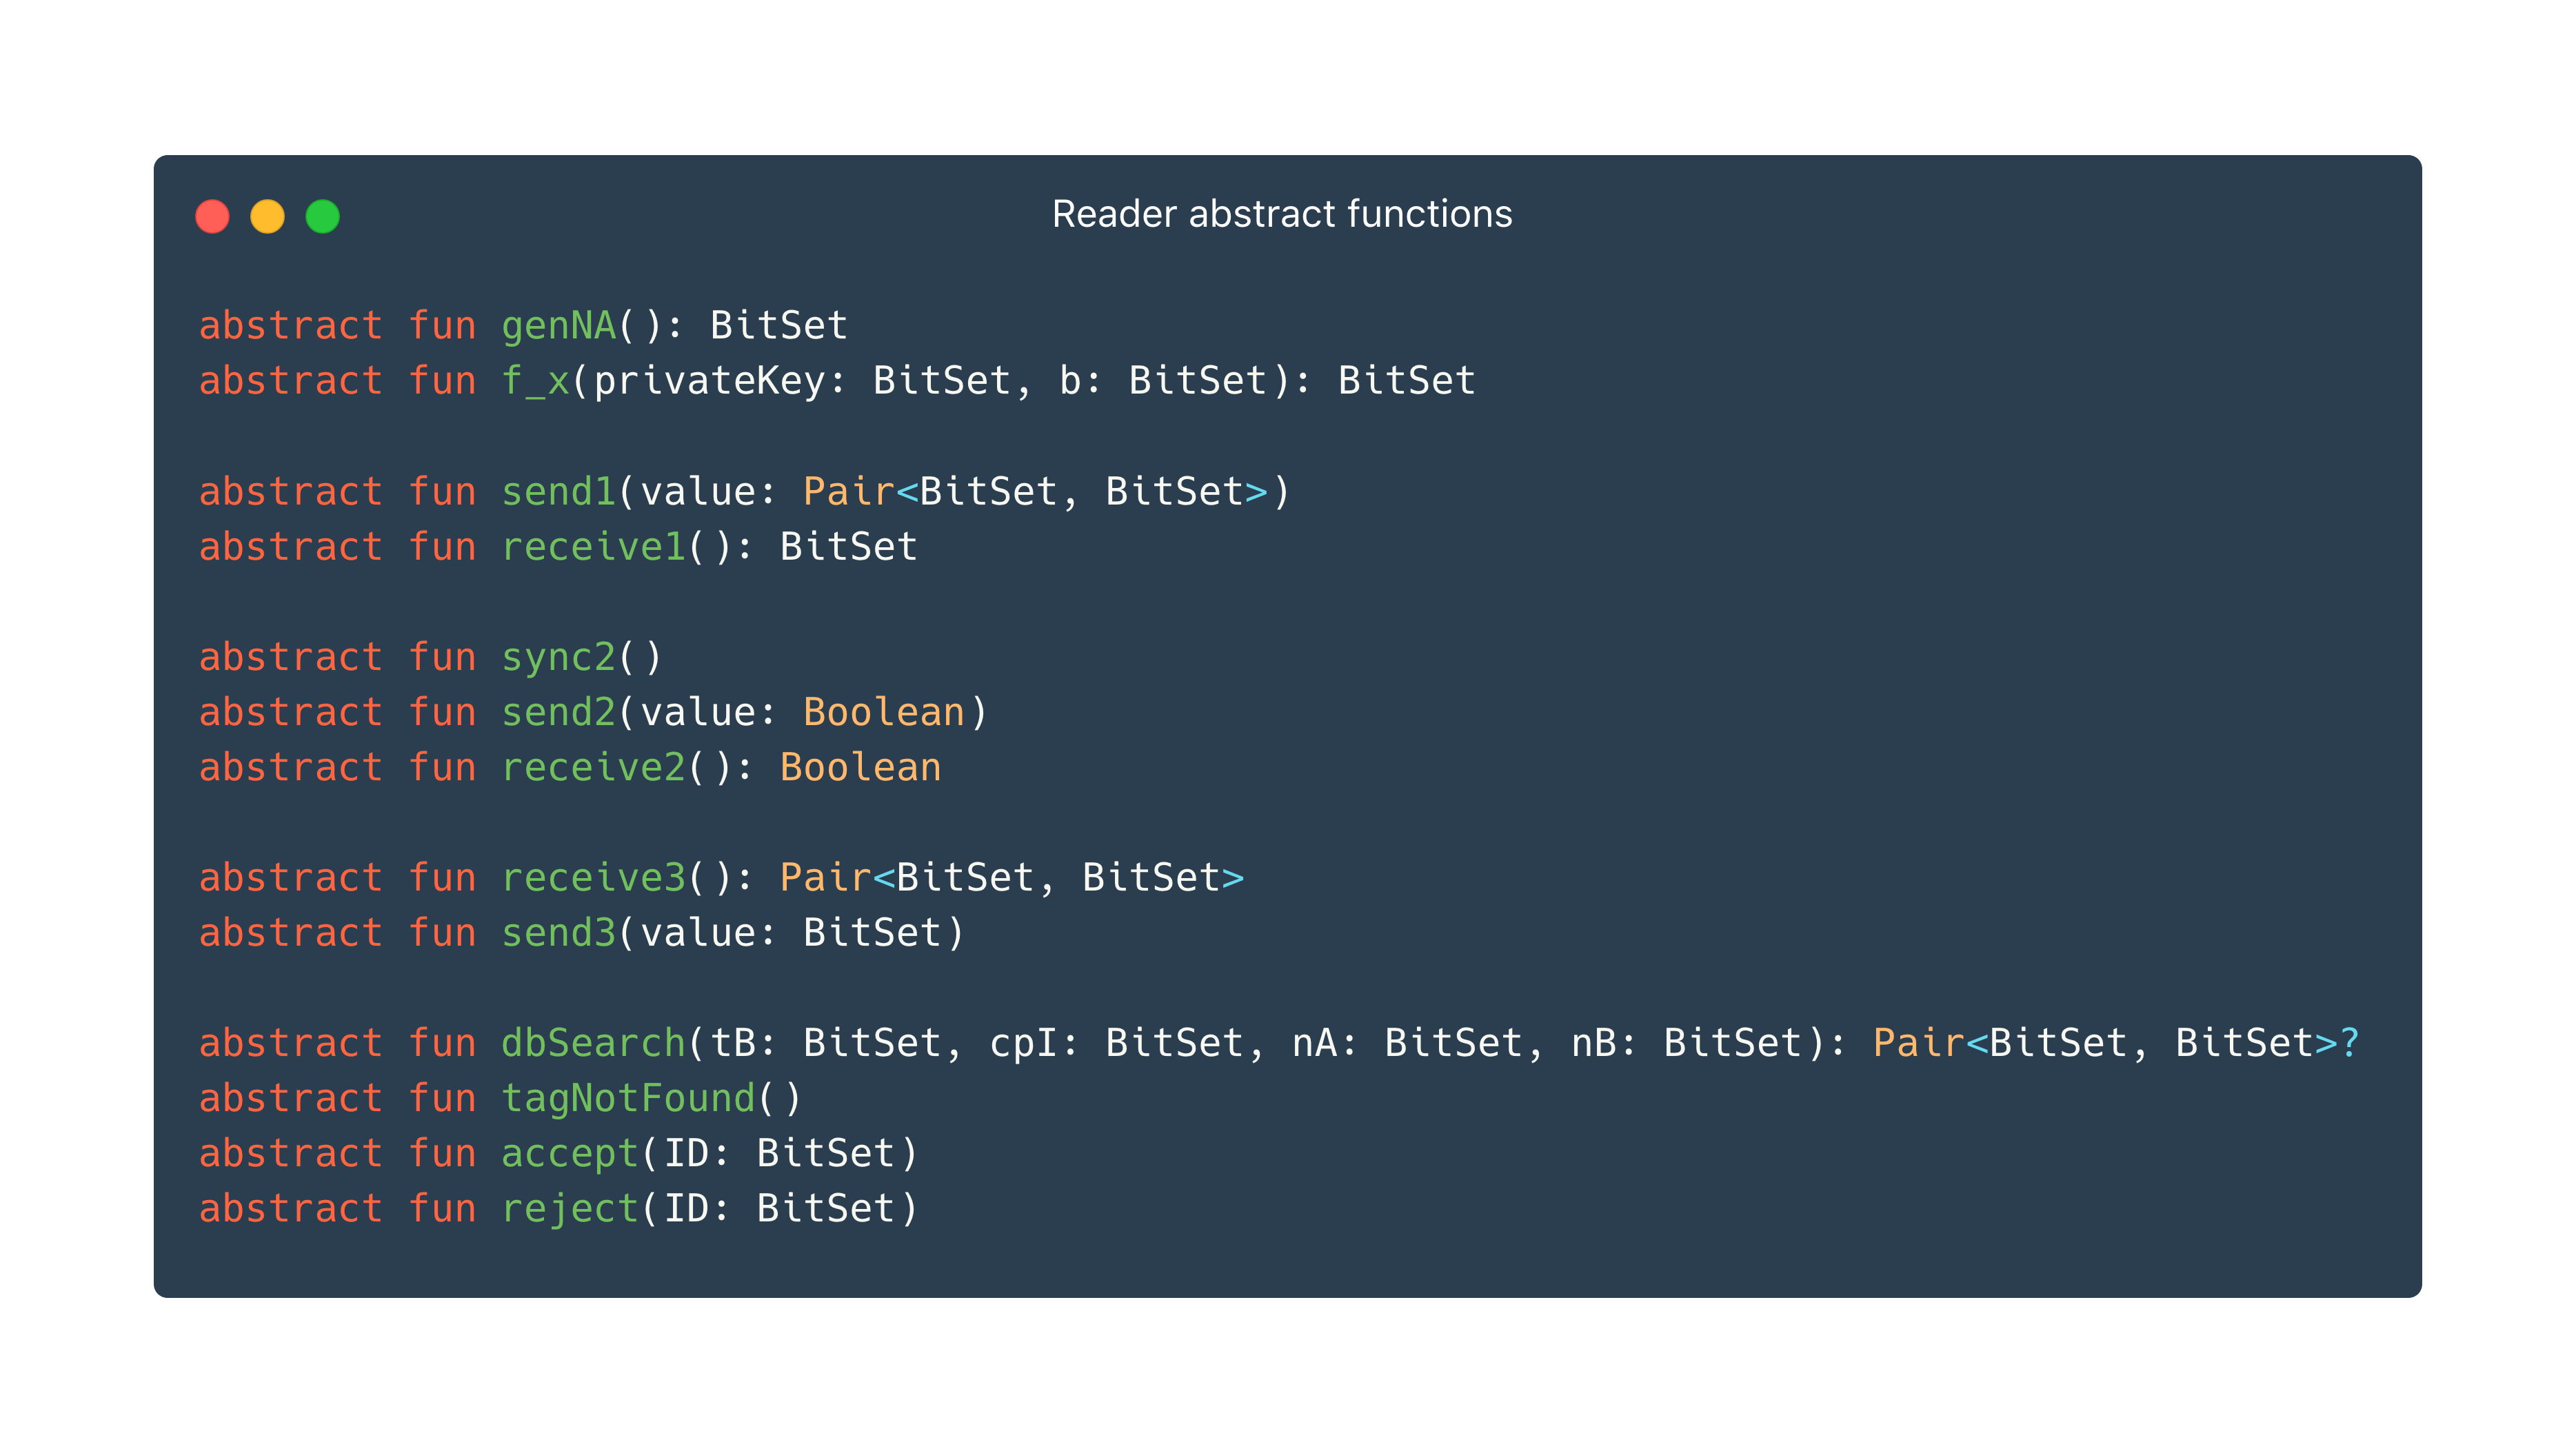
\includegraphics[width=.95\linewidth]{../assets/readerAbs}
\end{frame}

\begin{frame}{Librairie .jar : Test unitaire}
  LocalhostTest
\end{frame}

\begin{frame}{Librairie .jar : Utilisation}
  Comment on va utiliser la librairie : SKoWA
\end{frame}

\subsection{Application Android}

\begin{frame}{Application Android : Fonctionnalités}
  
  \begin{itemize}
    \item Voir ses cours de la journée
    \item Adhérer à la vérification de présence
    \item Effectuer le SKoWA
  \end{itemize}

\end{frame}

\begin{frame}{Maquette de l'application}
  \begin{adjustwidth}{-1.8em}{2em}
    \centering
    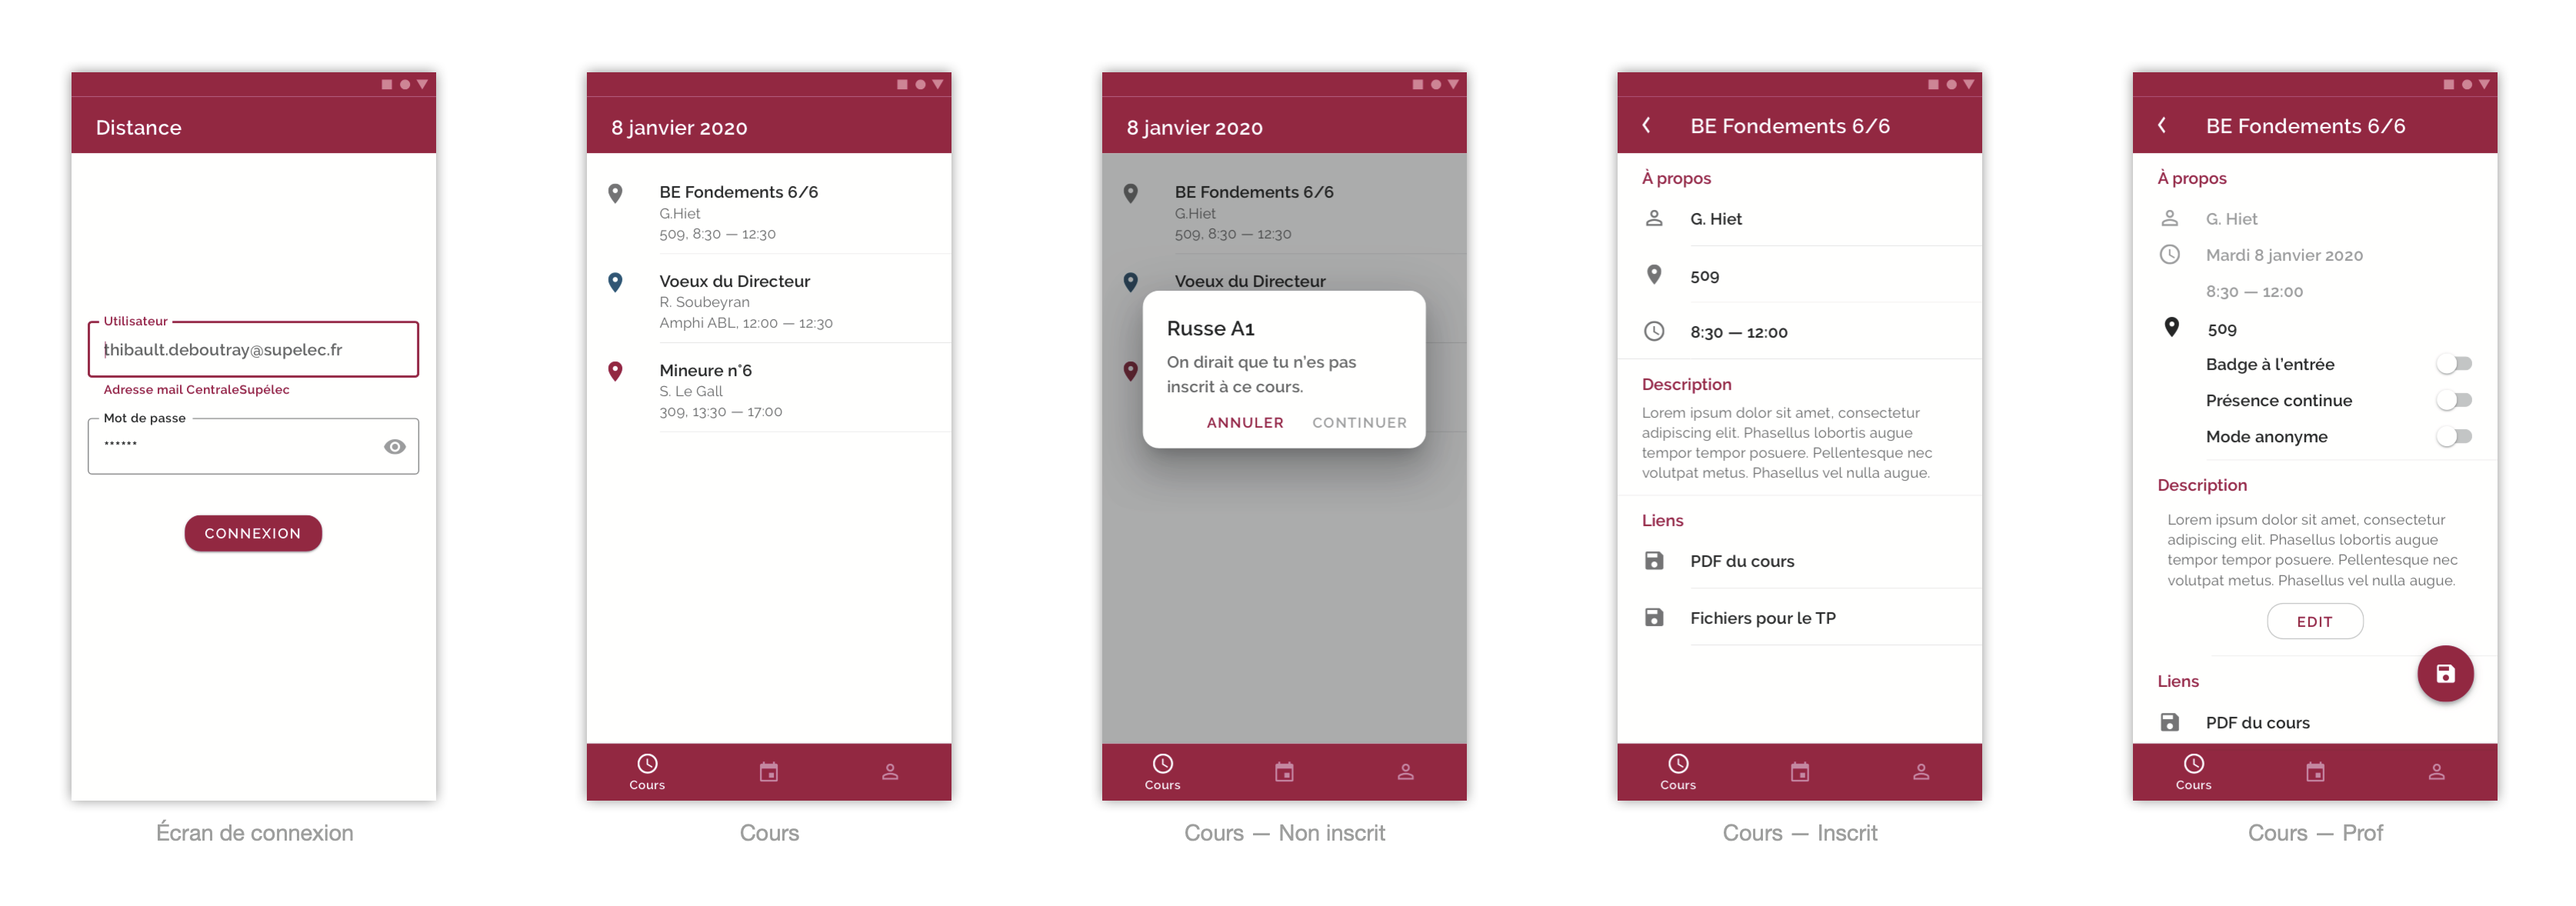
\includegraphics[width=1.1\linewidth]{../assets/maquette.png}
  \end{adjustwidth}
\end{frame}

\begin{frame}{App actuelle}
  
  \begin{itemize}
    \item Liste de cours (custom RecyclerView / Adapter)
    \item Test Audio
    \item SKoWA tag
  \end{itemize}

\end{frame}

\begin{frame}{Implémentation du Swiss-Knife}
  Détails de l'implémentation
\end{frame}

\subsection{SKoWA Reader}

\begin{frame}{SKoWA Reader : Fonctionnalités}
  
  \begin{itemize}
    \item Vérifier un tag
    \item Logs
  \end{itemize}

\end{frame}

\begin{frame}{Implémentation du Swiss-Knife}
  Détails de l'implémentation
\end{frame}

\begin{frame}{Traitement du signal}
  Détails de l'implémentation
\end{frame}

\begin{frame}{Résultats}
  Vidéo du SKoWA
\end{frame}

\section{Perspectives}

\section{Conclusion}


\begin{frame}{Références}
  \printbibliography
\end{frame}

% \section{Appendix}

% \section{Protocoles délimiteurs de distance}

% \subsection{Présentation}

% \begin{frame}{Les Protocoles délimiteurs de distance}
% Les Distance Bounding Protocols, ou Protocoles Délimiteurs de Distance, sont des protocoles de sécurité qui permettent à un vérificateur $V$ de s'assurer qu'un prouveur $P$ se trouve à une distance bornée et définie de lui-même. \cite{wiki:pdd}

% \bigskip

% \pause
% \begin{itemize}
% \item Introduits par Brands \& Chaum, en 1993 \cite{DB1}
% \item Détermine la borne supérieure de la distance avec un appareil
% \item Calculs basés sur la vitesse de déplacement d'une OEM (30 cm en 1 ns)
% \pause
% \item Problème : la vitesse de déplacement d'une OEM est proche de celle d'un calcul dans un CPU 
% \end{itemize}

% \end{frame}

% \subsection{Attaques}

% \begin{frame}{Attaques sur les protocoles délimiteurs de distance}

% En 2009, un article formalise les différentes attaques. \cite{attack}

% \medskip

% \begin{center}
% \begin{tikzpicture}
%     % Zone
%     \draw [black, thick, dotted] (0,0) circle [radius=2.25];

%     % Lecteur
%     \draw [fill] (0,0) circle [radius=0.05];
%     \node [above] at (0,0.2) {Lecteur};

%     \pause

%     % Distance fraud
%     \draw [fill, gray] (3,0) circle [radius=0.05];
%     \node [right, gray] at (3,0) {Tag};
%     \draw [->, thick, line width=1.2, gray] (2.75,0) -- (0.5,0);
%     \node [right, gray] at (4.5,2) {Distance fraud};

%     \pause

%     % Mafia fraud
%     \draw [fill, cyan] (1.32, -0.44) circle [radius=0.05];
%     \node [below, cyan] at (1.32, -0.54) {A};
%     \draw [fill, cyan] (3,-1) circle [radius=0.05];
%     \node [right, cyan] at (3,-1) {Tag};
%     \draw [->, thick, dashed, line width=1.2, cyan] (2.79,-0.93) -- (1.51,-0.5);
%     \draw [->, thick, line width=1.2, cyan] (1.1,-0.37) -- (0.47,-0.16);
%     \node [right, cyan] at (4.5,1) {Mafia fraud};

%     \pause

%     % Terrorist fraud
%     \draw [fill, orange] (1.32, 0.44) circle [radius=0.05];
%     \node [above, orange] at (1.32, 0.54) {A};

%     \draw [fill, orange] (3,1) circle [radius=0.05];
%     \node [right, orange] at (3,1) {Tag};
%     \draw [->, thick, dashed, line width=1.2, orange] (2.79,0.93) -- (1.51,0.5);
%     \draw [->, thick, line width=1.2, orange] (1.1,0.37) -- (0.47,0.16);
%     \node [right, orange] at (4.5,0) {Terrorist fraud};

%     \pause

%     % Impersonation fraud
%     \draw [red, thick] (-1.32,-0.44) circle [radius=0.3];
%     \node [below, red] at (-1.32, -0.74) {A};
%     \draw [fill, red] (-1.17,-0.44) circle [radius=0.05];
%     \draw [fill, red] (-1.32,-0.29) circle [radius=0.05];
%     \draw [fill, red] (-1.47,-0.44) circle [radius=0.05];
%     \draw [fill, red] (-1.32,-0.44) circle [radius=0.05];
%     \draw [fill, red] (-1.32,-0.59) circle [radius=0.05];
%     \draw [->, thick, line width=1.2, red] (-1.04,-0.35) -- (-0.47,-0.16);
%     \node [right, red] at (4.5,-1) {Impersonation fraud};

%     % Impersonation fraud
%     \draw [fill, olive] (-1.32, 0.44) circle [radius=0.05];
%     \node [above, olive] at (-1.32, 0.44) {A};
%     \draw [->, thick, line width=1.2, olive] (-1.1,0.37) -- (-0.47,0.16);
%     \node [right, olive] at (4.5,-2) {Impersonation fraud};

% \onslide<1->
% \end{tikzpicture}
% \end{center}

% \end{frame}

% \subsection{Un protocole : Swiss-Knife}

% \begin{frame}{Un protocole : Swiss-Knife}
%   Protocole délimiteur de distance proposé en 2008. \cite{SwissKnife}

%   \bigskip

%   \begin{itemize}
%     \item Authentification
%     \item Résistance aux mafia fraud et terrorist fraud
%     \item Faible complexité algorithmique
%     \item Faible taux de faux positifs
%     \item Confidentialité
%     \item Résistance aux erreurs
%   \end{itemize}

% \end{frame}


% \begin{frame}{Première phase : phase de préparation}
%   \begin{multicols}{2}
%     \begin{minipage}[c]{\linewidth}
%       \centering
%       \bigskip
%       \medskip
%       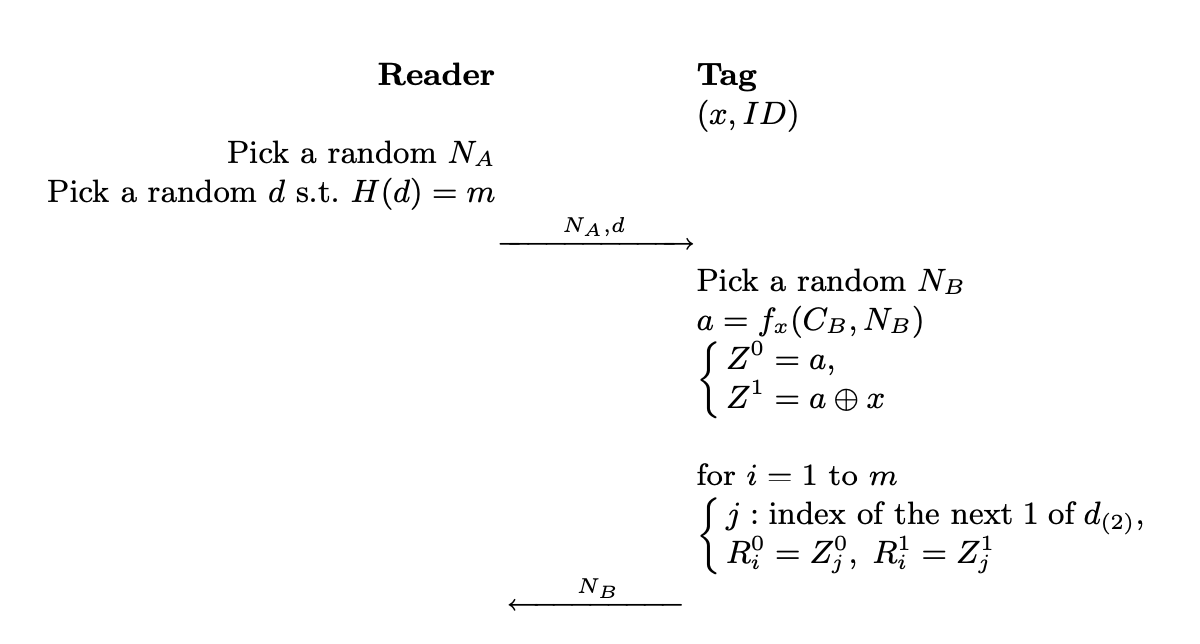
\includegraphics[width=\linewidth]{../assets/sk-phase1.png}
%     \end{minipage}

%     \begin{minipage}[t]{\linewidth}
%       \begin{enumerate}
%         \item Le lecteur choisit un nonce $N_A$, et $d$ un nombre avec $m$ bits 1.
%         \item Le tag choisit un nonce $N_B$, et calcule $a = f_x(C_B, N_B)$ avec sa clé secrète $x$ et $N_B$. ($C_B$ est une constante)
%         \item Le tag calcule $Z_0 = a$, $Z_1 = a \oplus x$. Il prépare ensuite les réponses possibles $R_0$ et $R_1$ selon le masque $d$.
%         \item Le tag envoie $N_B$ au lecteur.
%       \end{enumerate}
%     \end{minipage}
%   \end{multicols}
% \end{frame}

% \begin{frame}{Seconde phase : phase rapide}
%   \begin{multicols}{2}
%     \begin{minipage}[c]{\linewidth}
%       \centering
%       \bigskip
%       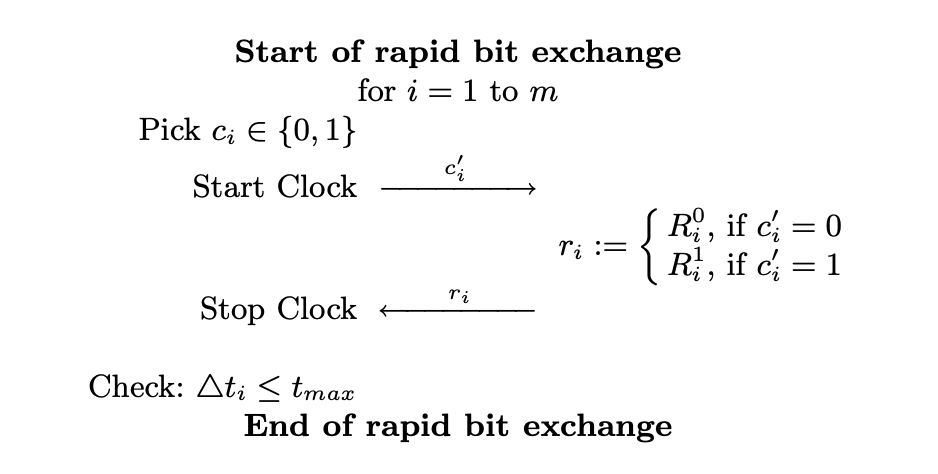
\includegraphics[width=\linewidth]{../assets/sk-phase2.png}
%     \end{minipage}

%     \begin{minipage}[t]{\linewidth}
%       \begin{enumerate}
%         \item Le lecteur envoie un bit aléatoire $c_i$, et démarre une horloge. Le tag reçoit $c_i'$ (possiblement incorrect).
%         \item Le tag répond $r'_i = R_i^{c'_i}$. Le lecteur reçoit $r_i$.
%         \item Le lecteur arrête l'horloge, et sauvegarde le délai associé $\Delta t_i$ et la réponse $r_i$ reçue.
%       \end{enumerate}
%     \end{minipage}
%   \end{multicols}
% \end{frame}

% \begin{frame}{Troisième phase : phase de vérification}
%   \begin{multicols}{2}
%     \begin{minipage}[c]{\linewidth}
%       \centering
%       \bigskip
%       \bigskip
%       \bigskip
%       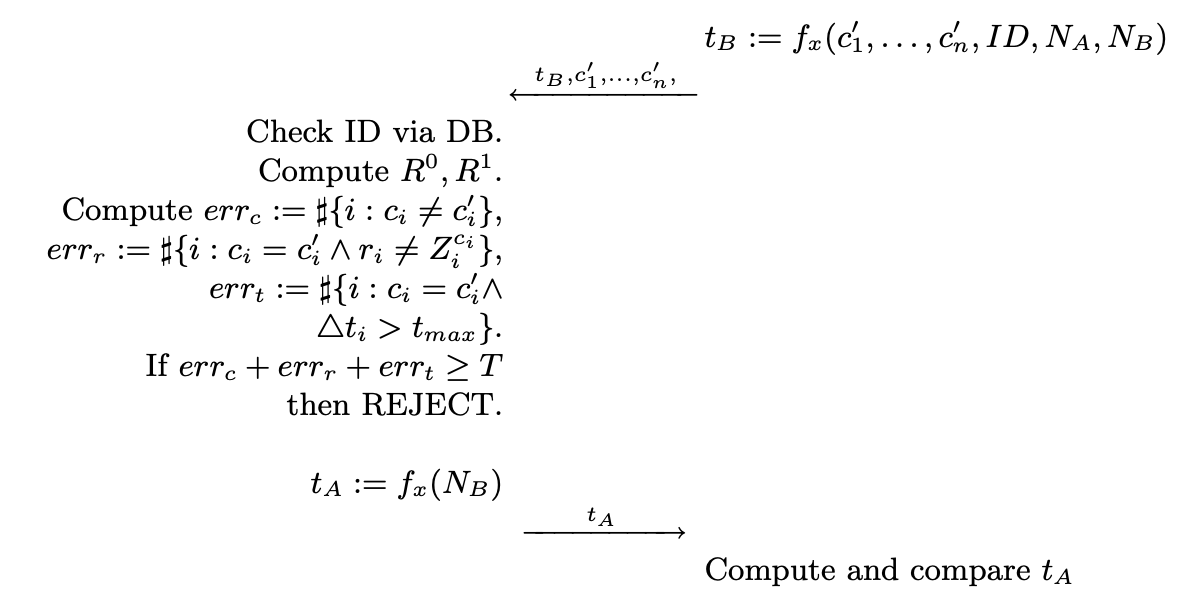
\includegraphics[width=\linewidth]{../assets/sk-phase3.png}
%     \end{minipage}

%     \begin{minipage}[t]{\linewidth}
%       \begin{enumerate}
%         \item Le tag envoie $t_B = f_x(c'_1, \hdots, c'_n, ID, N_A, N_B)$, et les $c'_i$.
%         \item Le lecteur cherche dans sa base de tags jusqu'à trouver $(ID, x)$ générant $t_B$.
%         \item Le lecteur calcule $R^0$ et $R^1$.
%         \item Le lecteur compte les erreurs, si il y en a plus de $T$, échec.
%         \item (optionnel) Le lecteur envoie $t_A := f_x(N_B)$ puis le tag le vérifie.
%       \end{enumerate}
%     \end{minipage}
%   \end{multicols}
% \end{frame}


% \begin{frame}{À venir...}
    
%   \begin{itemize}
%       \item Cycle de Développement itératif
%       \item Vérification par NFC    
%       \item Vérification sur la durée : phase rapide du Swiss-Knife par un autre vecteur que le Wi-Fi (Ultrason ?) afin d'assurer :
%       \begin{itemize}
%           \item La présence effective des utilisateurs dans la salle
%           \item Une compensation de la vitesse trop rapide du Wi-Fi et des collisions des paquets
%       \end{itemize}

%   \end{itemize}

% \end{frame}

\end{document}
